% 固定来源PDF印刷页52第2题四组选项图象的矢量示意重绘。
% 单调性、截距及渐近线忠于原页；曲线斜率和坐标比例仅作示意。
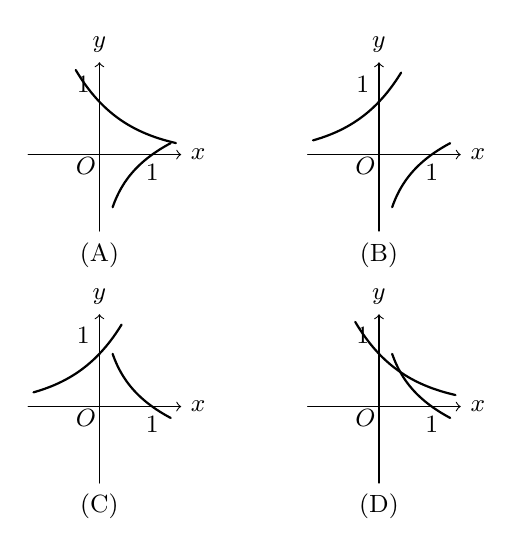
\begin{tikzpicture}[x=.67cm,y=.67cm,font=\small,line cap=round,line join=round]
  % (A) decreasing exponential and increasing logarithm.
  \begin{scope}
    \draw[->] (-1.35,0)--(1.55,0) node[right] {$x$};
    \draw[->] (0,-1.45)--(0,1.75) node[above] {$y$};
    \draw[thick,domain=-.45:1.45,samples=55,variable=\x] plot (\x,{exp(-1.05*\x)});
    \draw[thick,domain=.25:1.35,samples=55,variable=\x] plot (\x,{.72*ln(\x)});
    \node[below left,inner sep=1pt] at (0,0) {$O$};
    \node[above left] at (0,1) {$1$};
    \node[below] at (1,0) {$1$};
    \node at (0,-1.9) {(A)};
  \end{scope}

  % (B) increasing exponential and increasing logarithm.
  \begin{scope}[xshift=3.55cm]
    \draw[->] (-1.35,0)--(1.55,0) node[right] {$x$};
    \draw[->] (0,-1.45)--(0,1.75) node[above] {$y$};
    \draw[thick,domain=-1.25:.42,samples=55,variable=\x] plot (\x,{exp(1.05*\x)});
    \draw[thick,domain=.25:1.35,samples=55,variable=\x] plot (\x,{.72*ln(\x)});
    \node[below left,inner sep=1pt] at (0,0) {$O$};
    \node[above left] at (0,1) {$1$};
    \node[below] at (1,0) {$1$};
    \node at (0,-1.9) {(B)};
  \end{scope}

  % (C) increasing exponential and decreasing logarithm.
  \begin{scope}[yshift=-3.2cm]
    \draw[->] (-1.35,0)--(1.55,0) node[right] {$x$};
    \draw[->] (0,-1.45)--(0,1.75) node[above] {$y$};
    \draw[thick,domain=-1.25:.42,samples=55,variable=\x] plot (\x,{exp(1.05*\x)});
    \draw[thick,domain=.25:1.35,samples=55,variable=\x] plot (\x,{-.72*ln(\x)});
    \node[below left,inner sep=1pt] at (0,0) {$O$};
    \node[above left] at (0,1) {$1$};
    \node[below] at (1,0) {$1$};
    \node at (0,-1.9) {(C)};
  \end{scope}

  % (D) decreasing exponential and decreasing logarithm.
  \begin{scope}[xshift=3.55cm,yshift=-3.2cm]
    \draw[->] (-1.35,0)--(1.55,0) node[right] {$x$};
    \draw[->] (0,-1.45)--(0,1.75) node[above] {$y$};
    \draw[thick,domain=-.45:1.45,samples=55,variable=\x] plot (\x,{exp(-1.05*\x)});
    \draw[thick,domain=.25:1.35,samples=55,variable=\x] plot (\x,{-.72*ln(\x)});
    \node[below left,inner sep=1pt] at (0,0) {$O$};
    \node[above left] at (0,1) {$1$};
    \node[below] at (1,0) {$1$};
    \node at (0,-1.9) {(D)};
  \end{scope}
\end{tikzpicture}
